\begin{center}
{\textbf{Mercredi 18 août 2021 : Journée photo}}
\end{center}
\vspace{2mm}

Nouvelle journée, nouveaux cours.

Le matin, les groupes A et B apprennent à manier le deuxième outil-star de la géométrie : les triangles semblables, avec Pierre-Marie dans le groupe A, Martin et Anna dans le groupe B. Alexander instruit le groupe C sur les invariants, et Théo dirige un TD sur les polynômes et systèmes dynamiques modulo p dans le groupe D.

\begin{figure}[H]
\centering\includegraphics[width=6cm]{CR-18-0.jpg}\hspace{2cm}\includegraphics[width=6cm]{CR-18-1.jpg}
\caption{Le groupe A écoute attentivement Pierre-Marie tandis que les élèves du groupe B travaillent par petits groupes.}
\end{figure}

Un par un, les élèves sont photographiés par Tristan, qui passe tour à tour dans chaque groupe. Qui sait, peut-être que dans quelques années de nouveaux élèves iront chercher ces photos pour découvrir les têtes jeunes et innocentes de ceux qui seront devenus animatheurs ? En attendant, on on espère que le fond sera être au goût du très exigeant responsable poly, qui arrivera en deuxième période.

La deuxième partie de la journée est dédiée à l’algèbre dans les groupes A, B et D avec Domitille, Tristan, Théodore et Rémi. Les élèves du groupe C s’exercent en arithmétique avec Théo.

Une nouvelle rafraîchissante est annoncée en début d’après-midi. Les élèvent pourront aller à la piscine à la fin des cours ! Étonnamment, les listes des volontaires pour faire du sport ne se vident pas pour autant au profit de cette nouvelle opportunité. Un nombre de stagiaires encore plus important rejoint les terrains de volley et football à la fin des cours. Les joueurs s’affrontent avec une détermination et un professionnalisme toujours croissants.

\begin{figure}[H]
\centering\includegraphics[width=6cm]{CR-18-2.jpg}\hspace{2cm}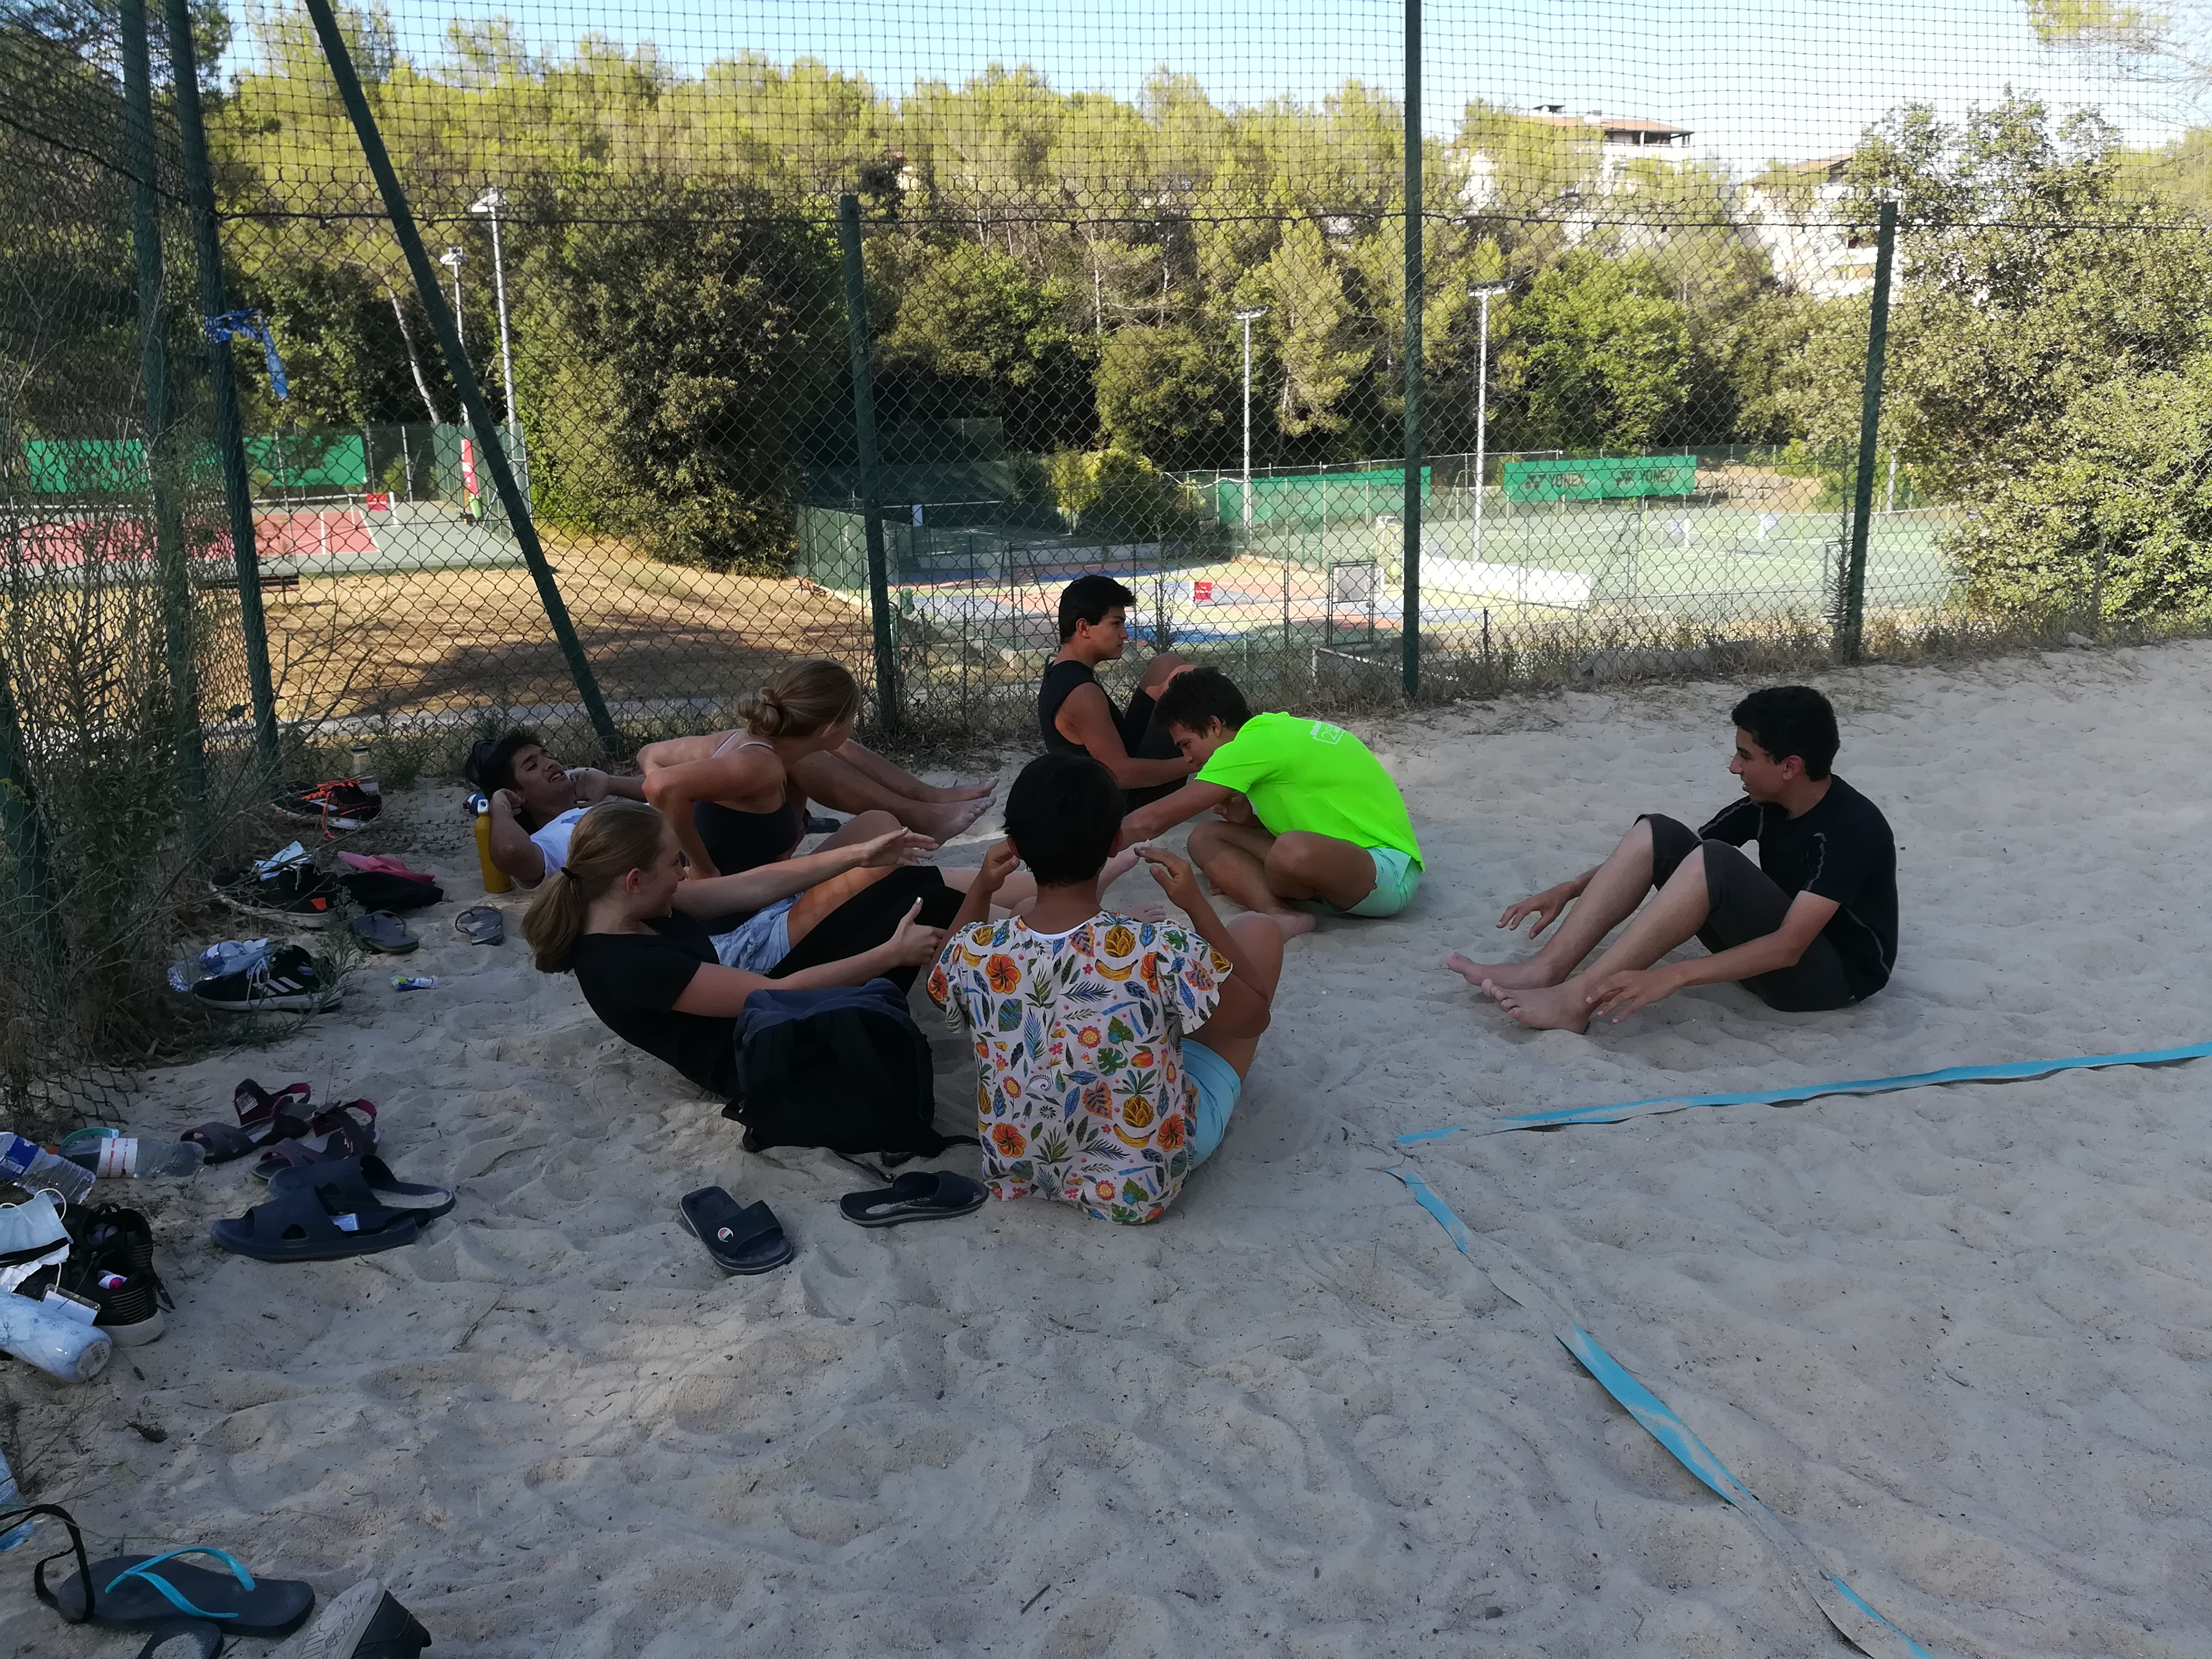
\includegraphics[width=6cm]{CR-18-4.jpg}
\caption{On se prépare à réceptionner le service choc de l’équipe adverse. Une partie de foot très dynamique.}
\end{figure}

Pendant ce temps, ceux qui ont décidé de se baigner profitent d’une piscine quasi vide.

Après ce riche deuxième jour de stage, tout le monde se rend à l’amphithéâtre pour la conférence de Raphaël sur la théorie de l’information. De \textit{Qui est-ce} à \textit{Code Names}, en passant par un tour de magie bluffant, Raphaël nous explique la définition mathématique de l’information, en nous entraînant jusqu’à l’entropie de Shannon.

\begin{figure}[H]
\centering\includegraphics[width=6cm]{CR-18-5.jpg}\hspace{2cm}\includegraphics[width=6cm]{CR-18-6.jpg}
\caption{Raphaël explique le logarithme. Les élèves mis à contribution !}
\end{figure}

Après la conférence s’organise un karaoké dans l’amphithéâtre, grand écran et micro sortis. Les plus grands classiques de la chanson française y passent, Céline Dion, Goldman, Sardou et tant d’autres, mais sans oublier les classiques internationaux avec Lady Gaga ou encore Taylor Swift. Évidemment, on ne passe pas à côté des grands classiques Disney pour chanter, hurler, ou parfois les deux, dans le micro.

\begin{figure}[H]
\centering\includegraphics[width=7cm]{CR-18-7.jpg}
\end{figure}

Et, fatigués, les élèves vont se coucher pour faire de beaux rêves bleus.

